\documentclass[border=8pt]{standalone}
\usepackage{tikz}
\usetikzlibrary{quantikz2,positioning,arrows.meta,calc,shapes.geometric,decorations.pathreplacing}
\usepackage{mathpazo}
\usepackage{amsmath,amssymb,braket}
\definecolor{qxblue}{HTML}{156082}
\definecolor{qxink}{HTML}{0B1A22}
\definecolor{qxtint}{HTML}{E4EEF3}
\definecolor{qxsand}{HTML}{F5ECD7}
\definecolor{qxrose}{HTML}{F6DEDE}
\definecolor{qxsage}{HTML}{E2EFE3}
\tikzset{g/.style={fill=qxtint,draw=qxink}, o/.style={fill=qxsand,draw=qxink}, e/.style={fill=qxrose,draw=qxink},
  q/.style={fill=qxsage,draw=qxink},
  grp/.style={dashed,rounded corners,draw=qxblue!80,inner xsep=4pt},
  box/.style={draw=qxink,rounded corners=3pt,fill=qxtint,align=center,inner sep=6pt,font=\small},
  arr/.style={-{Stealth[length=2.2mm]},thick,draw=qxink}}
\begin{document}

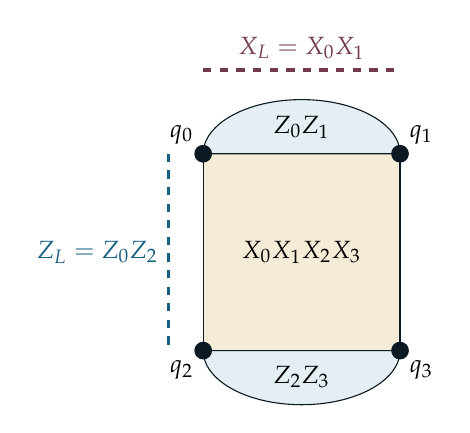
\begin{tikzpicture}[scale=1.25, every node/.style={font=\small}]
\fill[qxsand,draw=qxink] (0,0) rectangle (2,2);
\node at (1,1) {$X_0X_1X_2X_3$};
\fill[qxtint,draw=qxink] (0,2) arc (180:0:1 and 0.55) -- cycle;
\node at (1,2.27) {$Z_0Z_1$};
\fill[qxtint,draw=qxink] (2,0) arc (0:-180:1 and 0.55) -- cycle;
\node at (1,-0.27) {$Z_2Z_3$};
\foreach \p/\l in {(0,2)/0,(2,2)/1,(0,0)/2,(2,0)/3}{\fill[qxink] \p circle (0.09); }
\node[above left] at (0,2) {$q_0$}; \node[above right] at (2,2) {$q_1$};
\node[below left] at (0,0) {$q_2$}; \node[below right] at (2,0) {$q_3$};
\draw[qxblue,very thick,dashed] (-0.35,2) -- (-0.35,0) node[midway,left]{$Z_L=Z_0Z_2$};
\draw[qxblue!60!red,very thick,dashed] (0,2.85) -- (2,2.85) node[midway,above]{$X_L=X_0X_1$};
\end{tikzpicture}

\end{document}
